% !TEX root = ../../presentation.tex

\begin{slide}{Hardware Layer}
  \begin{tikzpicture}
    \pause
    \node [inner sep=0] (cpu) at (-2.5, 0)
          {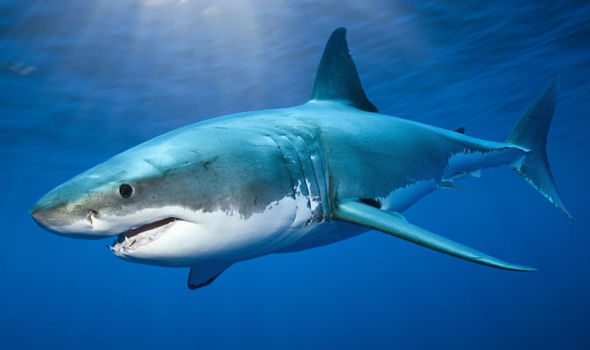
\includegraphics[width=4cm, height=2.2cm]{shark}};
    \draw [white, rounded corners=5pt, line width=5pt]
        (cpu.north west) --
        (cpu.north east) --
        (cpu.south east) --
        (cpu.south west) -- cycle;
    \draw (cpu)+(0, -1.4) node {\textbf{CPU}};

    \pause
    \node [inner sep=0] (gpu) at (+2.5, 0)
          {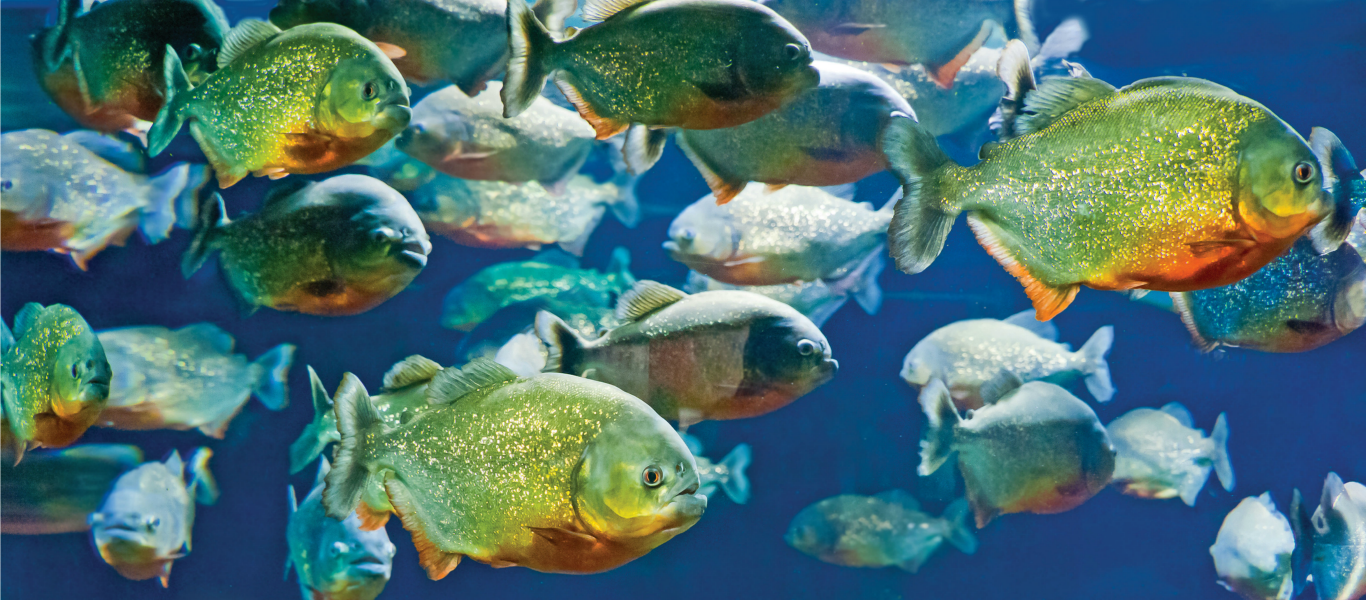
\includegraphics[width=4cm, height=2.2cm]{piranha}};
    \draw [white, rounded corners=5pt, line width=5pt]
        (gpu.north west) --
        (gpu.north east) --
        (gpu.south east) --
        (gpu.south west) -- cycle;
    \draw (gpu)+(0, -1.4) node {\textbf{GPU}};

    \pause
    \node [inner sep=0] (asic) at (0, -3.5)
      {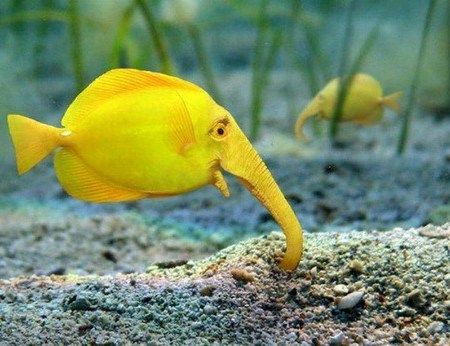
\includegraphics[scale=0.25, trim={0 2cm 0 0.5cm}, clip]{weird-fish}};
    \draw [white, rounded corners=5pt, line width=5pt]
        (asic.north west) --
        (asic.north east) --
        (asic.south east) --
        (asic.south west) -- cycle;
    \draw (asic)+(0, -1.5) node {\textbf{ASIC}};
  \end{tikzpicture}
\end{slide}

\begin{slide}{GPUs}
  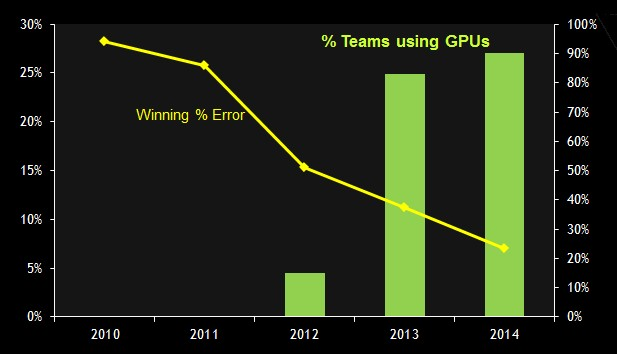
\includegraphics[scale=0.4]{imagenet-gpu}

  \vspace{0.3cm}
  \small
  Teams using GPUs at ImageNet Competition
\end{slide}

\begin{slide}{GPUs}
  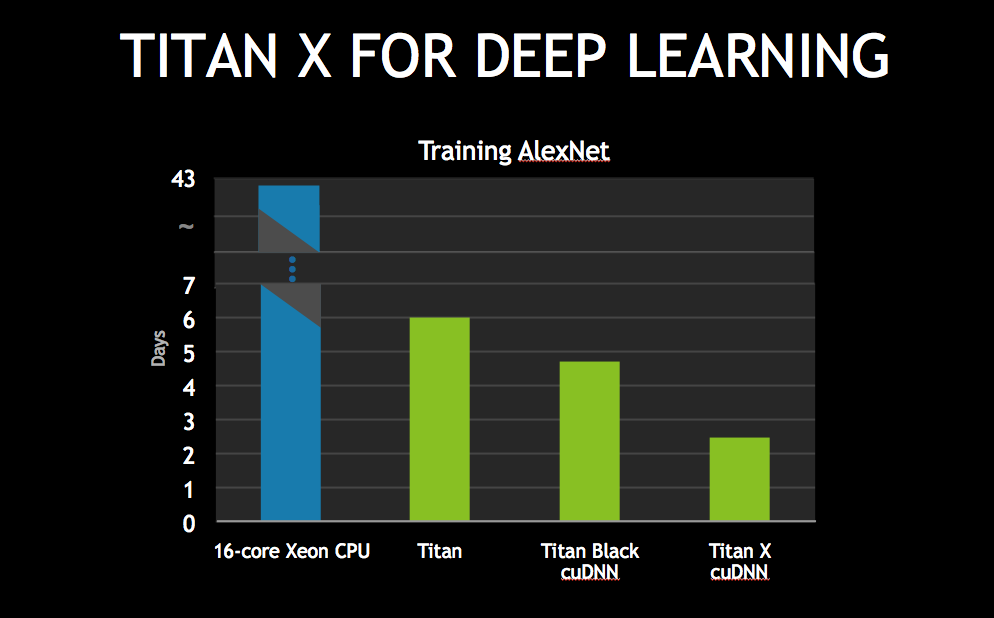
\includegraphics[scale=0.5]{alexnet-training-days}

    \vspace{0.3cm}
    \small
    Training Time for ImageNet
\end{slide}

\begin{slide}{GPUs}
  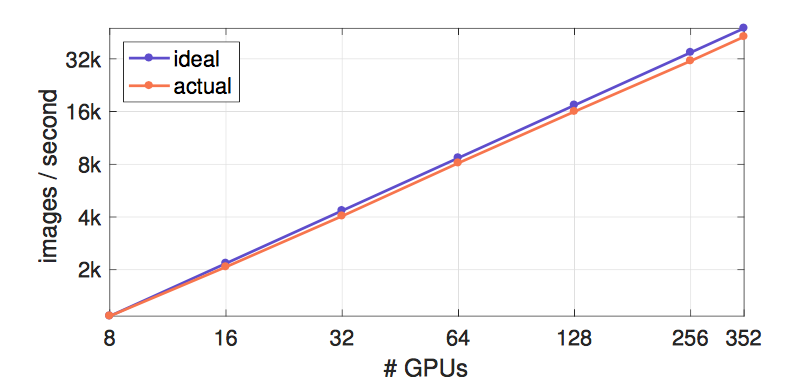
\includegraphics[scale=0.35]{fb-scaling}

    \vspace{0.3cm}
    \small
    Accurate, Large Minibatch SGD: Training ImageNet in 1 Hour

    \vspace{0.1cm}
    Goyal et al. (2017)
\end{slide}

% \begin{slide}{GPUs}
%   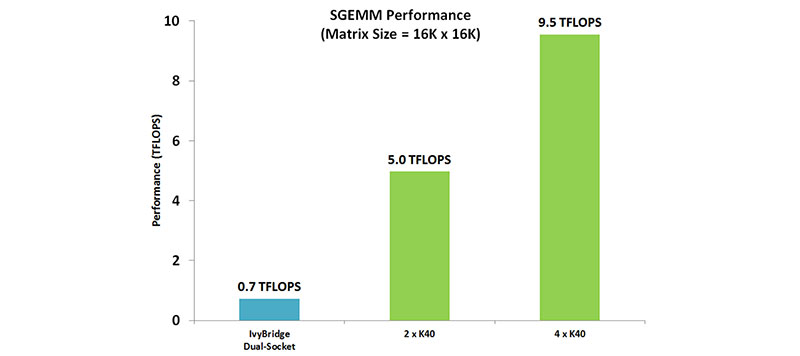
\includegraphics[scale=0.37]{sgemm}
%
%     \vspace{0.3cm}
%     \small
%     Single Precision General Matrix/Matrix Multiply Performance
% \end{slide}

\begin{slide}{}
  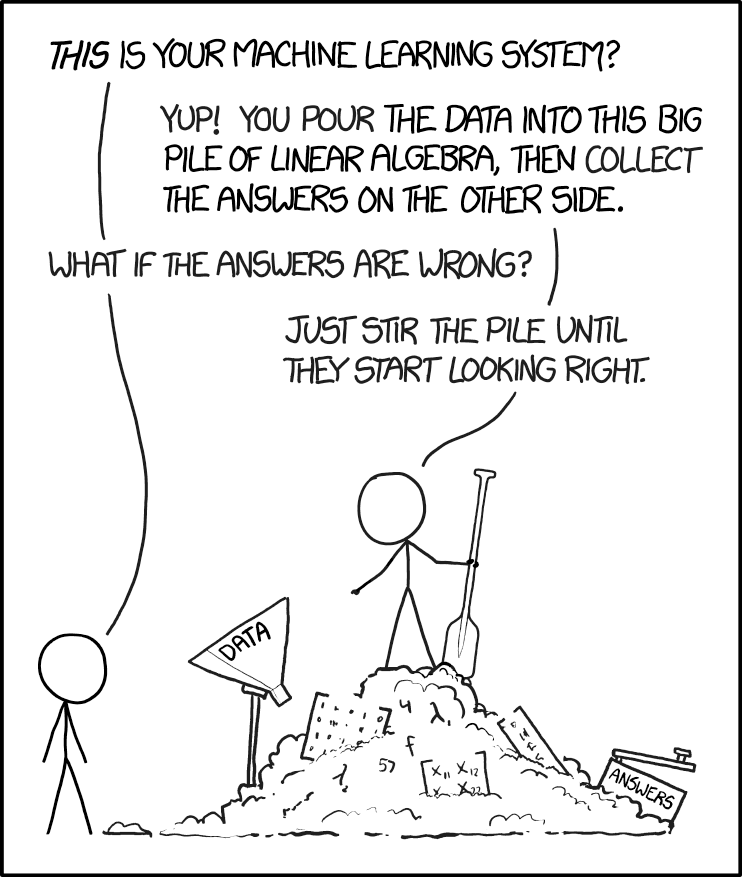
\includegraphics[scale=0.22]{xkcd}
\end{slide}
